\section{Background}
\label{sec:background}

Radio searches for technosignatures began at centimetre wavelengths and
have largely stayed there. The first targeted experiments
\citep{CocconiMorrison1959,Drake1960}, the programmes reviewed by
\citet{Tarter2001} and Project Phoenix \citep{Backus2002} all worked
below a few gigahertz. The modern generation divides into targeted and
commensal surveys at centimetre and metre wavelengths
\citep{Zhang2020,Czech2021,Morrison2023,FAST3IATLAS2025,LOFARdualsite2023},
with wide-field low-frequency coverage from the MWA \citep{Tremblay2024}
and single-dish C- and K-band work at 6 and 18\,GHz with the Sardinia
Radio Telescope \citep{SRT2025}. Machine-learning interference rejection
is now central to that effort
\citep{Ma2023,Choza2024,GLOBULAR2025,AnomalyParkesGBT2025,BRaTs2026}. The
classical threshold search used here lacks that capability, and instead
uses a spatial test on the star against control positions in the same
field, which a single dish cannot make.

Above about 30\,GHz the record is nearly empty, and that is what makes
this frequency range new. ALMA observes in Bands~3 to~10, spanning
roughly 84 to 950\,GHz; of those eight bands, one has been searched for
technosignatures. For continuity with the centimetre literature we note
one familiar power scale: the Arecibo planetary radar radiated
$\AreciboW$\,W at \ArecGHz\,GHz
\citep{Drake1974,EarthDetectingEarth2025}. It carries no transmitter
model into the millimetre band, where an aperture of that diameter is not
realisable, so the benchmark used in \S\ref{sec:discussion} is instead a
dish of \BenchDiam\,m.

\citet{Mason2025} is the only prior millimetre search and the only
comparable archival one. They searched Band~3 windows toward
\MasonNStar{} Gaia~DR3 stars lying in the fields of \MasonNCal{} ALMA
calibrators, observed for other science and so usable for free. Their
nearest target is at \MasonNearKpc\,kpc, where a $5\sigma$ threshold
corresponds to EIRP$_{\rm min}>{}$\MasonNearEirp\,W. Their targets are
four orders of magnitude more distant than ours, so an EIRP ratio between
the two surveys would be almost entirely a distance term. The quantity
that does not depend on distance is the minimum detectable \emph{received}
flux, $F_{\rm min}=S_{\rm min}\,\delta\nu$. It must be quoted at a matched
channel width, because $S_{\rm min}$ falls as $\delta\nu^{-1/2}$ while
$F_{\rm min}$ rises as $\delta\nu^{1/2}$. Mason
et~al.\ reach \MasonFluxLo--\MasonFluxHi\,W\,m$^{-2}$ across their four
fields, on a \MasonChanKHz\,kHz channel at a bare $5\sigma$ threshold. On
that same channel width and the same threshold convention, the
fine-channel windows searched here reach \FluxMatchBest\,W\,m$^{-2}$ at
best, a factor \FluxBestRatio{} deeper, and \FluxMatchMed\,W\,m$^{-2}$ at
the median, a factor \FluxMedRatio{} shallower. The two experiments are
therefore comparable in depth and differ in what they cover: distant
stars in four calibrator fields, against \NStars{} stars within 40\,pc
over a frequency range reaching about nine times higher. They also
identified the obstacles that shape the present method: drift rates scale
with frequency, smearing erodes sensitivity unless drift is searched for,
and the dense forest of molecular lines raises the confusion background.
Every window reported here was re-reduced and re-searched from the raw
archive data with the pipeline of \S\ref{sec:method}, so for any star in
common the numbers to cite are this paper's.

Figure~\ref{fig:context}(a) places this survey among published searches,
in minimum detectable EIRP against distance. The vertical axis is
physically commensurable: for a carrier narrower than every programme's
channel, the minimum detectable EIRP is a total radiated power and not a
spectral power density, so the same quantity is plotted for each
programme. What differs is the convention. The value plotted for this
survey is $\mathrm{EIRP}_{90}$, a 90 per cent recovery through the
complete automated selection, whereas most published limits are nominal
thresholds at which recovery is not stated; the comparison runs against
us. Any EIRP advantage toward the nearest systems is a $d^{2}$ effect and
not an instrumental one. Panel~(b) shows the other axis that matters.
Archived correlator channels here span about seven orders of magnitude in
width, and all of them are far coarser than a dedicated narrowband
backend. The distinctive feature of this survey is therefore its
frequency regime and its channelisation, not its depth. It also samples
far fewer stars and far fewer epochs than a dedicated search, and
complements those programmes rather than deepening them.

\begin{figure}
\centering
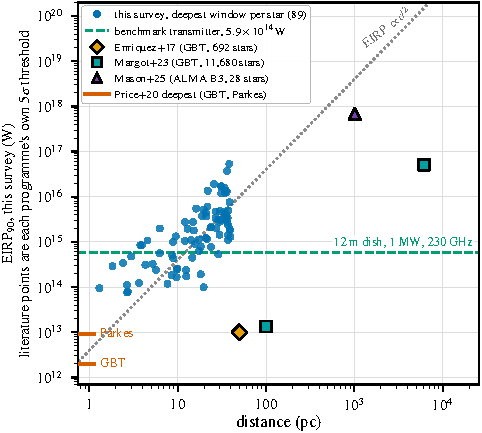
\includegraphics[width=\columnwidth]{figures/eirp_context_a.pdf}\\
{\footnotesize (a)}\\[4pt]
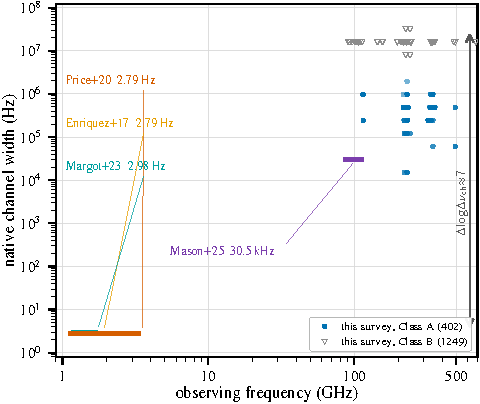
\includegraphics[width=\columnwidth]{figures/eirp_context_b.pdf}\\
{\footnotesize (b)}
\caption{Where this survey sits among published radio technosignature
searches. \textbf{(a)} Minimum detectable EIRP against distance: blue,
this survey, the deepest window per star; orange, \citet{Enriquez2017};
aqua, \citet{Margot2023}; violet, \citet{Mason2025}; left-edge ticks,
\citet{Price2020}. Grey dotted, EIRP $\propto d^{2}$ at constant received
flux; green dashed, the \BenchDiam\,m benchmark transmitter of
\S\ref{sec:discussion}. The ordinates are commensurable as total powers
for a sub-channel carrier; what differs between programmes is the
detection threshold and the completeness level each adopts, and this
survey's value is the stricter of the two conventions.
\textbf{(b)} Native channel width against observing frequency for every
searched window (filled, Class~A; open, Class~B), with the
comparison programmes as horizontal segments. The channel widths span
about seven orders of magnitude, which is what the
$\Delta\log\Delta\nu_{\rm ch}\approx7$ annotation marks: the
channelisation, not the plotted power, is what differs most between
programmes.}
\label{fig:context}
\end{figure}

A non-detection becomes a quantitative statement only through a stated
search volume. \citet{Wright2018} formalised that volume, and
\citet{Margot2023} its conversion into an upper bound on the fraction of
stars hosting a transmitter; \citet{EarthDetectingEarth2025} asked where
Earth's own technosignatures would be detectable. Such a bound is valid
only if the sample represents the population it is meant to describe.
This sample was assembled by other observers for other purposes, so it
does not, and \S\ref{sec:sample} states what it is instead.

%% REQUEST (results owner, sections/05_results.tex): \ref{fig:context} in
%% "nominal trigger thresholds span ... at a median of" means the EIRP
%% panel. Please write Fig.~\ref{fig:context}(a).
%% REQUEST (stack-discussion owner, sections/06_discussion.tex): two
%% changes. (i) \ref{fig:context} in "the novelty is the frequency regime
%% and not depth" means the channel-width panel: please write
%% Fig.~\ref{fig:context}(b). (ii) The matched-received-flux comparison
%% with Mason et al. has moved into \S\ref{sec:background}, where the
%% prior work is introduced; please delete it from \S6 and cite
%% \S\ref{sec:background} instead, so it is made once. The macros
%% \FluxSelMatchMed and \FluxSelMedRatio are then unused and may go.
%% REQUEST (stack-discussion owner): \S\ref{sec:discussion} is the single
%% place the \BenchDiam-m benchmark is evaluated against the sample; this
%% section points at it and must not be the place the comparison is made.
%% REQUEST (appendix-triage owner): sections/app_E_notation.tex holds
%% fig:contextapp, which is panel (a) of the merged float above. Please
%% delete that float and its label; it is now cited as
%% Fig.~\ref{fig:context}(a) from here. \ref{fig:context} in
%% sections/app_D_externalchecks.tex ("the threshold distribution is") and
%% both citations in sections/app_F_freqconventions.tex mean panel (a) and
%% need the panel letter.
%% REQUEST (figures owner): figures/eirp_context_a.pdf still carries the
%% Arecibo line, which this section now makes in prose and must not also
%% make as a line. Please replot it with the \BenchDiam-m benchmark
%% instead, and plot the survey's points at the adopted sensitivity.
%% REQUEST (abstract-intro owner): your requests (i) and (ii) are done --
%% the physical-motivation sentence and the bare "below ~30 GHz" claim are
%% gone from here. \S2 now substantiates the band-by-band statement
%% instead of asserting it, so please keep \S1's version to one clause.
%% The haystack fraction occurs only in \S1.
